\chapter{Charges supersymétriques, fermeture et superspace}

\lectureoverview{La supersymétrie est difficile, non pas parce que ses règles sont nombreuses, mais parce qu’elles réunissent des idées que la physique ordinaire tient séparées. Nous commencerons par les variables de Grassmann, dont les éléments impairs anticommutent et dont les fonctions s’arrêtent après un nombre fini de termes. L’algèbre de leurs dérivées fournit ensuite le modèle des générateurs de symétrie impairs. Un oscillateur bosonique et un oscillateur fermionique donnent les charges supersymétriques les plus simples : leur anticommutateur est le Hamiltonien, si bien que l’échange des bosons et des fermions est indissociable d’une translation dans le temps. La même algèbre peut être représentée géométriquement par des translations dans les directions de Grassmann d’un espace-temps élargi appelé superspace.}

\section{Pourquoi revenir en arrière avant d’avancer}

La supersymétrie est l’une des constructions les plus abstraites de la physique. Comme les rotations et les translations, elle est une symétrie, mais elle ne s’inscrit pas dans l’espace-temps ordinaire sans élargir le sens que nous donnons au mot coordonnée. Ses paramètres naturels sont des quantités de Grassmann : des objets que l’on peut additionner et multiplier, mais qui anticommutent au lieu de commuter.

C’est pourquoi s’attaquer directement à l’algèbre finale ne serait pas utile. Nous commencerons par rendre l’arithmétique impaire maniable, puis nous rappellerons comment s’organisent les symétries continues ordinaires, avant de réunir ces deux idées. Le chemin est plus long, mais chaque étape prépare la suivante.

\section{L’algèbre de Grassmann en pratique}

\subsection{Éléments pairs et impairs}

Soit \(\epsilon_i\) des générateurs indépendants de Grassmann. Ils vérifient
\begin{equation}
\epsilon_i\epsilon_j=-\epsilon_j\epsilon_i,
\qquad
\{\epsilon_i,\epsilon_j\}=0.
\end{equation}
En posant \(i=j\), on obtient
\begin{equation}
2\epsilon_i^2=0,
\qquad
\epsilon_i^2=0,
\end{equation}
sur les nombres réels ou complexes. Le générateur n’est pas nul ; seul son carré est nul.

Chaque élément homogène a une parité. Un produit contenant un nombre impair de générateurs de Grassmann est impair, tandis qu’un produit qui en contient un nombre pair est pair :
\begin{align}
\text{odd}\times\text{odd}&=\text{even},\\
\text{odd}\times\text{even}&=\text{odd},\\
\text{even}\times\text{even}&=\text{even}.
\end{align}
Les éléments pairs commutent avec les éléments homogènes. Deux éléments impairs anticommutent. Ainsi,
\begin{equation}
n\epsilon_i=\epsilon_i n,
\qquad
\epsilon_i\epsilon_j=-\epsilon_j\epsilon_i,
\end{equation}
lorsque \(n\) est pair.

Un élément pair n’est pas nécessairement un nombre réel ou complexe ordinaire. Le produit
\(\epsilon_1\epsilon_2\), par exemple, est pair et nilpotent. Les nombres ordinaires constituent la partie scalaire de l’algèbre, tandis que les produits pairs fournissent d’autres éléments commutants.

\begin{classroomqa}
\audiencequestion{Y a-t-il une différence entre l’algèbre de Grassmann et les nombres de Grassmann, ou s’agit-il de la même chose ? \lecturetimestamp{00:06:45}}
\lecturerresponse{Les éléments sont les nombres de Grassmann ; l’algèbre est l’ensemble de ces éléments, muni de ses règles d’addition et de multiplication. On peut donc parler, de façon approximative, d’un même objet, mais il est utile de distinguer les objets que l’on manipule des règles qui régissent ces manipulations.}
\end{classroomqa}

\subsection{Les fonctions s’arrêtent}

Une fonction d’une variable de Grassmann ne comporte que deux puissances possibles :
\begin{equation}
f(\epsilon)=a+b\epsilon.
\end{equation}
Il n’y a pas de terme en \(\epsilon^2\). Avec deux générateurs indépendants,
\begin{equation}
f(\epsilon_1,\epsilon_2)
=a+b_1\epsilon_1+b_2\epsilon_2+c\epsilon_1\epsilon_2.
\end{equation}
le développement s’arrête dès que les deux générateurs sont apparus. Pour \(n\) générateurs indépendants, les monômes ordonnés forment une base de dimension \(2^n\) :
\begin{equation}
1,\quad
\epsilon_i,\quad
\epsilon_i\epsilon_j,\quad
\ldots,\quad
\epsilon_1\epsilon_2\cdots\epsilon_n.
\end{equation}
\editorialnote{L’énoncé général selon lequel la dimension est finie et vaut \(2^n\) est le prolongement des exemples à un et deux générateurs. On peut aussi définir une algèbre de Grassmann infinie, mais chacun des polynômes utilisés ici ne fait intervenir qu’un nombre fini de générateurs.}

Lorsque deux générateurs réels sont réunis en une paire complexe \(\theta,\bar\theta\), une fonction générale peut s’écrire, pour un ordre choisi,
\begin{equation}
f(\theta,\bar\theta)
=a+\bar b\,\theta+\bar\theta\,b+c\,\bar\theta\theta.
\end{equation}
La barre indique la notation en paire complexe employée ici. Inverser l’ordre des deux derniers facteurs change le signe :
\begin{equation}
\bar\theta\theta=-\theta\bar\theta.
\end{equation}

Il est généralement commode d’attribuer une parité déterminée à la fonction entière. Si \(f\) est pair, alors \(a\) et \(c\) sont pairs, tandis que \(b\) et \(\bar b\) sont impairs. Si \(f\) est impair, ces parités sont inversées. Les coefficients peuvent eux-mêmes appartenir à une algèbre de Grassmann plus grande, à condition de ne pas dépendre des variables particulières par rapport auxquelles on développe.

\begin{classroomqa}
\audiencequestion{Peut-on introduire une variable de Grassmann dans des fonctions trigonométriques ou d’autres fonctions analytiques ? \lecturetimestamp{00:11:06}}
\lecturerresponse{Oui, mais le développement en série s’arrête immédiatement. Pour un générateur impair,
\[
\sin\epsilon=\epsilon,\qquad
\cos\epsilon=1,\qquad
e^\epsilon=1+\epsilon.
\]
Les appellations usuelles subsistent, mais il y a trop peu de puissances pour que les fonctions acquièrent leur complexité analytique habituelle.}
\end{classroomqa}

\section{La dérivation, une question de signes}

Nous utilisons une dérivée de Grassmann à gauche. Ses règles locales définissantes sont
\begin{equation}
\partial_\theta a=0,
\qquad
\partial_\theta(\theta B)=B,
\end{equation}
lorsque \(a\) et \(B\) ne dépendent pas de \(\theta\). Avant de dériver, déplaçons le \(\theta\) concerné vers la gauche. Chaque passage au travers d’un autre facteur impair change le signe.

Par exemple, si \(b\) est impair,
\begin{equation}
b\theta=-\theta b,
\qquad
\partial_\theta(b\theta)=-b.
\end{equation}
La dérivée n’a rien de mystérieux. Le signe moins est apparu avant la dérivation, lors de la permutation des facteurs impairs.

\subsection{Le calcul à deux variables}

Revenons à
\begin{equation}
f(\theta,\bar\theta)
=a+\bar b\,\theta+\bar\theta\,b+c\,\bar\theta\theta.
\end{equation}
Supposons d’abord que \(f\) soit pair. Alors \(\bar b\) est impair et \(c\) est pair. En réordonnant les termes qui contiennent \(\theta\),
\begin{align}
\bar b\,\theta&=-\theta\bar b,\\
c\,\bar\theta\theta&=-\theta c\,\bar\theta.
\end{align}
On obtient donc
\begin{equation}
\partial_\theta f=-\bar b-c\bar\theta.
\end{equation}

Si \(f\) est impair, alors \(\bar b\) est pair et \(c\) est impair. Le premier terme ne traverse aucun coefficient impair, tandis que le dernier \(\theta\) traverse deux facteurs impairs, \(c\) et \(\bar\theta\). Les deux signes se compensent :
\begin{equation}
\partial_\theta f=\bar b+c\bar\theta.
\end{equation}

\begin{classroomqa}
\audiencequestion{Pourquoi les deux termes qui subsistent portent-ils tous deux un signe moins dans l’exemple pair ? \lecturetimestamp{00:16:49}}
\lecturerresponse{Le premier signe vient du passage de \(\theta\) au-delà du coefficient impair \(\bar b\). Dans le dernier terme, \(c\) est pair, mais \(\theta\) doit passer au-delà de la variable impaire \(\bar\theta\). Chaque permutation croise un facteur impair et produit donc un signe moins.}
\end{classroomqa}

La réponse dépend de la convention d’ordre, mais pas les mathématiques. Si nous étions partis de \(c\theta\bar\theta\) plutôt que de \(c\bar\theta\theta\), le coefficient affiché aurait différé d’un signe et la formule de dérivation aurait changé en conséquence.

\begin{classroomqa}
\audiencequestion{Le dernier terme aurait-il pu s’écrire avec \(\theta\) et \(\bar\theta\) dans l’ordre inverse, et le signe obtenu a-t-il une signification plus profonde ? \lecturetimestamp{00:18:50}}
\lecturerresponse{On peut l’écrire dans l’un ou l’autre ordre, mais l’échange des deux variables impaires change le signe. On peut absorber ce signe dans le coefficient \(c\). À ce stade, il s’agit d’une règle de calcul : l’ordre compte, la parité ne change pas, et un changement de signe ne transforme jamais un objet impair en objet pair. Cette règle prend toute son importance physique lorsque le même calcul impose la statistique fermionique et la supersymétrie.}
\end{classroomqa}

\begin{classroomqa}
\audiencequestion{Les coefficients \(a,b,c\) proviennent-ils simplement du corps des nombres complexes ? \lecturetimestamp{00:20:47}}
\lecturerresponse{Ils peuvent être des nombres complexes ordinaires lorsque leur parité doit être paire, mais ils peuvent aussi contenir des générateurs autres que \(\theta,\bar\theta\). L’algèbre considérée comprend normalement tous les scalaires complexes, ainsi qu’un ensemble choisi de générateurs impairs et leurs produits.}
\end{classroomqa}

\begin{classroomqa}
\audiencequestion{Les dérivées des fonctions paires et impaires semblent opposées. Est-ce une symétrie générale ? \lecturetimestamp{00:22:31}}
\lecturerresponse{Pas à elle seule. Les signes découlent mécaniquement de la parité de chaque coefficient et du nombre de facteurs impairs traversés. Il arrive que deux réponses soient opposées, mais la règle fiable est plus simple : chaque échange de deux objets impairs produit un signe moins.}
\end{classroomqa}

\subsection{La coordonnée et la dérivée comme opérateurs}

Il existe une analogie ordinaire instructive. Faisons agir la multiplication par \(x\) et la dérivation par \(x\) sur une fonction arbitraire \(g(x)\). Alors
\begin{align}
\partial_x\!\left(xg\right)&=g+xg',\\
x\partial_xg&=xg',
\end{align}
d’où
\begin{equation}
[\partial_x,x]g=g.
\end{equation}
Comme cela vaut pour toute \(g\),
\begin{equation}
[\partial_x,x]=1.
\end{equation}
Avec \(p=-i\partial_x\), on retrouve l’algèbre position-impulsion habituelle, dans les unités où \(\hbar=1\).

L’analogue de Grassmann fait intervenir un anticommutateur. Prenons
\begin{equation}
f(\theta)=a+\theta b,
\end{equation}
avec \(a\) pair et \(b\) impair, de sorte que \(f\) soit pair. D’abord,
\begin{equation}
\theta\partial_\theta f=\theta b.
\end{equation}
Dans l’ordre inverse,
\begin{align}
\partial_\theta(\theta f)
&=\partial_\theta(\theta a+\theta^2b)\\
&=a.
\end{align}
En additionnant les deux ordres, on retrouve la fonction initiale :
\begin{equation}
\left(\partial_\theta\theta+\theta\partial_\theta\right)f
=a+\theta b=f.
\end{equation}
Ainsi,
\begin{equation}
\boxed{\{\partial_\theta,\theta\}=1.}
\end{equation}
La dérivée \(\partial_\theta\) est elle-même impaire. C’est pourquoi sa relation canonique avec la coordonnée impaire est un anticommutateur.

\begin{classroomqa}
\audiencequestion{Peut-on utiliser une fonction qui comporte à la fois des parties paires et impaires, au lieu de lui attribuer une parité déterminée ? \lecturetimestamp{00:31:05}}
\lecturerresponse{On peut former de tels éléments inhomogènes, mais les calculs s’organisent normalement autour d’objets homogènes pairs et impairs. Une parité déterminée rend univoque chaque signe dans un produit gradué ; un objet mixte se traite en le décomposant en ses parties paire et impaire.}
\end{classroomqa}

\begin{classroomqa}
\audiencequestion{La fonction test \(g(x)\) du calcul du commutateur ordinaire était-elle supposée impaire ? \lecturetimestamp{00:31:45}}
\lecturerresponse{Non. C’était une fonction ordinaire d’une coordonnée ordinaire commutative. Elle servait uniquement à montrer comment démontrer l’identité d’opérateurs \([\partial_x,x]=1\) avant de reprendre le raisonnement avec la paire de Grassmann \(\partial_\theta,\theta\).}
\end{classroomqa}

\begin{classroomqa}
\audiencequestion{Le nombre de générateurs indépendants de Grassmann est-il limité ? \lecturetimestamp{00:32:16}}
\lecturerresponse{Il n’existe aucune limite algébrique supérieure. Pour \(n\) générateurs, la base compte \(2^n\) monômes, si bien que les calculs se compliquent rapidement, mais la construction elle-même fonctionne pour tout \(n\) fini.}
\end{classroomqa}

\subsection{Intégration}

L’intégrale sur une variable de Grassmann est définie par
\begin{equation}
\int d\theta\,1=0,
\qquad
\int d\theta\,\theta=1.
\end{equation}
Par conséquent, pour \(f(\theta)=a+\theta b\),
\begin{equation}
\int d\theta\,f(\theta)=b=\partial_\theta f(\theta).
\end{equation}
L’intégration et la dérivation extraient donc la même composante. C’est l’intégrale de Berezin. Sa normalisation est le choix simple unique compatible avec l’invariance par translation et l’intégration par parties de Grassmann. \editorialnote{Les règles sur les composantes précisent l’affirmation du cours selon laquelle l’intégration et la dérivation de Grassmann sont une seule et même opération.}

\section{La symétrie ordinaire comme référence}

Considérons un groupe unitaire continu de générateurs hermitiens \(G_i\). Au voisinage de l’identité,
\begin{equation}
U(\alpha)=\mathbf 1+i\alpha^iG_i+O(\alpha^2),
\end{equation}
où les \(\alpha^i\) sont des paramètres commutatifs ordinaires. La loi de multiplication infinitésimale est encodée par l’algèbre de Lie
\begin{equation}
[G_i,G_j]=i f_{ij}{}^{k}G_k.
\end{equation}
Les constantes \(f_{ij}{}^k\) sont les constantes de structure. La fermeture signifie que le commutateur de deux générateurs quelconques est une combinaison linéaire de générateurs déjà présents dans l’algèbre.

Pour les rotations,
\begin{equation}
[L_i,L_j]=i\varepsilon_{ijk}L_k.
\end{equation}
Les trois composantes hermitiennes peuvent être combinées en opérateurs d’échelle non hermitiens
\begin{equation}
L_\pm=L_x\pm iL_y,
\end{equation}
qui augmentent ou diminuent de une unité le nombre quantique magnétique \(m\). Les combinaisons complexes sont utiles sans que l’hermiticité des générateurs physiques sous-jacents soit modifiée.

Dans une base générale, seuls les deux premiers indices de \(f_{ij}{}^k\) doivent être antisymétriques. Pour une algèbre compacte munie d’une métrique orthonormée invariante, on peut abaisser le dernier indice et choisir des conventions telles que \(f_{ijk}\) soit totalement antisymétrique, comme c’est le cas pour les rotations. \editorialnote{Cette précision distingue l’antisymétrie universelle du commutateur de la propriété plus forte que l’on peut obtenir dans la base usuelle des rotations.}

Pour que \(G_i\) engendre une véritable symétrie d’un système indépendant du temps,
\begin{equation}
[H,G_i]=0.
\end{equation}
De façon équivalente, \(G_i\) laisse invariant chaque sous-espace propre de l’énergie. En l’absence de dépendance temporelle explicite, l’équation de Heisenberg donne
\begin{equation}
\frac{dG_i}{dt}=i[H,G_i]=0,
\end{equation}
le générateur est donc une charge conservée.

Les observables ordinaires sont paires. Un champ fermionique est impair, mais un champ impair isolé n’est pas en lui-même une observable mesurable ; les opérateurs physiques contiennent un nombre total pair de facteurs fermioniques. La supersymétrie change la parité des générateurs, et non celle qu’exigent les résultats observables.

La notation qui convient dans tous les cas est le commutateur gradué
\begin{equation}
[X,Y]_{\mathrm{gr}}
=XY-(-1)^{|X||Y|}YX.
\end{equation}
C’est un commutateur ordinaire si l’un des opérateurs est pair, et un anticommutateur si les deux sont impairs.

\section{L’oscillateur supersymétrique le plus simple}

\subsection{Un mode bosonique et un mode fermionique}

Considérons un mode bosonique unique, avec les opérateurs de création et d’annihilation \(a_+\) et \(a_-\) :
\begin{equation}
[a_-,a_+]=1,
\qquad
[a_+,a_+]=[a_-,a_-]=0.
\end{equation}
Son opérateur nombre est
\begin{equation}
N_B=a_+a_-,
\end{equation}
et son nombre d’occupation peut prendre les valeurs \(0,1,2,\ldots\).

Pour un mode fermionique unique, introduisons \(c_+\) et \(c_-\) :
\begin{equation}
\{c_-,c_+\}=1,
\qquad
\{c_+,c_+\}=\{c_-,c_-\}=0.
\end{equation}
Il en résulte que
\begin{equation}
c_+^2=c_-^2=0,
\qquad
N_F=c_+c_-,
\end{equation}
et que le nombre d’occupation ne peut valoir que \(0\) ou \(1\). Les opérateurs bosoniques sont pairs, les opérateurs fermioniques sont impairs, et chaque \(a_\pm\) commute avec chaque \(c_\pm\).

\editorialnote{La nilpotence limite le mode fermionique à un seul état occupé. Le mode bosonique, lui, admet un nombre d’occupation illimité ; une brève affirmation contraire dans la discussion en classe est contredite par l’algèbre de l’oscillateur elle-même.}

Supposons que le boson et le fermion aient la même énergie au repos \(m\), et définissons
\begin{equation}
Q=\sqrt m\,a_+c_-,
\qquad
\bar Q=Q^\dagger=\sqrt m\,a_-c_+.
\end{equation}
L’opérateur \(Q\) annihile un fermion et crée un boson. Son conjugué annihile un boson et crée un fermion. Chacun contient un opérateur fermionique et est donc impair.

Sur les états de nombre, leur action est explicite :
\begin{align}
Q\ket{n,1}
&=\sqrt{m(n+1)}\,\ket{n+1,0},
&
Q\ket{n,0}&=0,\\
\bar Q\ket{n,0}
&=\sqrt{mn}\,\ket{n-1,1},
&
\bar Q\ket{n,1}&=0.
\end{align}
\editorialnote{Les formules sur les états de nombre donnent directement, avec la normalisation appropriée, l’action de remplacement de particule décrite dans le cours.}

\subsection{L’anticommutateur se ferme sur l’énergie}

L’analogue gradué de la recherche d’une algèbre de Lie consiste à calculer
\begin{align}
\{Q,\bar Q\}
&=Q\bar Q+\bar Q Q\\
&=m\left(a_+c_-a_-c_+
        +a_-c_+a_+c_-\right).
\end{align}
Comme les \(a\) sont pairs, ils traversent les \(c\) sans produire de signe :
\begin{equation}
\{Q,\bar Q\}
=m\left(a_+a_-c_-c_+
        +a_-a_+c_+c_-\right).
\end{equation}
Utilisons maintenant
\begin{equation}
c_-c_+=1-c_+c_-,
\qquad
a_-a_+=a_+a_-+1.
\end{equation}
On obtient alors
\begin{align}
\{Q,\bar Q\}
&=m\left[
N_B(1-N_F)+(N_B+1)N_F
\right]\\
&=m(N_B+N_F).
\end{align}
Le facteur deux supplémentaire apparu provisoirement pendant la réorganisation à l’oral disparaît : une contribution fournit \(N_B\), l’autre fournit \(N_F\).

Pour des particules au repos de masses égales, le Hamiltonien est
\begin{equation}
H=m(N_B+N_F).
\end{equation}
Ainsi,
\begin{equation}
\boxed{\{Q,\bar Q\}=H.}
\end{equation}

\begin{figure}[H]
\centering
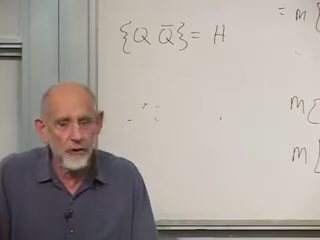
\includegraphics[width=0.62\textwidth]{lecture_05_figure_02.png}
\lectureframe{00:55:46.300}
\caption{La relation de fermeture centrale isolée au tableau. Les accolades et \(Q,\bar Q,H\) sont visibles ; la virgule est implicite dans la notation usuelle de l’anticommutateur.}
\end{figure}

Le zéro de l’énergie a été choisi de sorte que l’état vide ait \(H=0\). Dans l’oscillateur supersymétrique, c’est la convention naturelle : les contributions bosonique et fermionique d’énergie du point zéro se compensent. \editorialnote{Le cours travaille directement avec l’énergie totale au repos et ne fait pas apparaître séparément les termes d’énergie du point zéro ; la convention énoncée explicite ce choix.}

Le Hamiltonien est pair. C’est aussi un générateur de symétrie : il engendre les translations dans le temps. Les générateurs impairs ne se ferment donc pas entre eux sans que l’on inclue le générateur pair des translations temporelles.

\begin{classroomqa}
\audiencequestion{Lequel des éléments de la relation est pair ? Est-ce le Hamiltonien ? \lecturetimestamp{00:58:24}}
\lecturerresponse{Oui. L’énergie est une observable ordinaire, donc \(H\) est pair. La charge supersymétrique \(Q\) est impaire, et le produit de deux quantités impaires est pair ; \(\{Q,\bar Q\}\) peut donc être égal à \(H\). Des générateurs pair et impair sont liés par un commutateur, et non par un anticommutateur.}
\end{classroomqa}

\subsection{Compléter l’algèbre}

Les relations entre éléments de même parité sont immédiates :
\begin{equation}
\{Q,Q\}=2Q^2=0,
\qquad
\{\bar Q,\bar Q\}=2\bar Q^2=0,
\end{equation}
car \(Q^2\) contient \(c_-^2\) et \(\bar Q^2\) contient \(c_+^2\).

Il reste à établir la relation avec \(H\). Posons
\begin{equation}
H\ket{E}=E\ket{E}.
\end{equation}
Si les masses du boson et du fermion sont égales, \(Q\) remplace l’un par l’autre sans changer l’énergie. Par conséquent, \(Q\ket{E}\) est soit nul, soit un autre état propre associé à la même valeur propre :
\begin{equation}
H Q\ket{E}=E Q\ket{E}.
\end{equation}
D’autre part,
\begin{equation}
QH\ket{E}=Q(E\ket{E})=E Q\ket{E}.
\end{equation}
En soustrayant,
\begin{equation}
[H,Q]\ket{E}=0.
\end{equation}
Si les états propres de l’énergie forment une base complète, cette relation vaut comme identité d’opérateurs :
\begin{equation}
[H,Q]=0,
\qquad
[H,\bar Q]=0.
\end{equation}

\begin{classroomqa}
\audiencequestion{Que se passe-t-il si le boson et le fermion n’ont pas la même masse ? \lecturetimestamp{01:01:16}}
\lecturerresponse{Le remplacement de l’un par l’autre change alors l’énergie ; la charge supersymétrique proposée ne commute donc pas avec le Hamiltonien, et la supersymétrie simple disparaît. Pour
\[
H=m_BN_B+m_FN_F,
\]
le résultat explicite est
\[
[H,Q]=(m_B-m_F)Q.
\]
Il s’annule précisément lorsque \(m_B=m_F\). \editorialnote{Le commutateur pour des masses inégales donne directement sous forme d’opérateur l’argument fondé sur le changement d’énergie, et explicite la condition d’égalité des masses.}}
\end{classroomqa}

\begin{classroomqa}
\audiencequestion{Peut-on reprendre plus lentement l’argument fondé sur les états propres de l’énergie ? \lecturetimestamp{01:01:37}}
\lecturerresponse{Partons de \(H\ket{E}=E\ket{E}\). L’égalité des masses implique que \(Q\ket{E}\) possède la même énergie déterminée \(E\), donc \(HQ\ket{E}=EQ\ket{E}\). Dans l’ordre inverse, on obtient \(QH\ket{E}=QE\ket{E}=EQ\ket{E}\), puisque \(E\) est un scalaire ordinaire. La différence s’annule sur chaque état propre de l’énergie. La complétude permet alors d’étendre cette affirmation de ces états à l’équation d’opérateurs \([H,Q]=0\).}
\end{classroomqa}

L’algèbre complète de ce modèle est donc
\begin{align}
\{Q,\bar Q\}&=H,\\
\{Q,Q\}&=\{\bar Q,\bar Q\}=0,\\
[H,Q]&=[H,\bar Q]=0.
\end{align}
Les charges supersymétriques sont des charges impaires conservées. Plus étonnant encore, leur algèbre mêle une opération qui change le type de particule au générateur d’une translation de l’espace-temps.

\section{Pourquoi le Hamiltonien représente une translation temporelle}

Dans ce modèle dépouillé, il n’y a pas de coordonnée spatiale, mais il y a le temps. L’équation de Schrödinger s’écrit
\begin{equation}
i\frac{\partial}{\partial t}\ket{\psi(t)}
=H\ket{\psi(t)}.
\end{equation}

\begin{figure}[H]
\centering
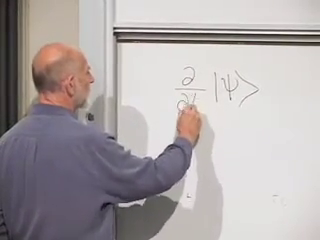
\includegraphics[width=0.56\textwidth]{lecture_05_figure_03.png}
\lectureframe{01:07:26.300}
\caption{La dérivée temporelle écrite à côté de \(\ket{\psi}\). La main masque une partie du dénominateur ; l’équation de Schrödinger complète est donnée ci-dessus.}
\end{figure}

Pour un décalage fini \(\delta\),
\begin{equation}
\ket{\psi(t+\delta)}
=e^{-iH\delta}\ket{\psi(t)}.
\end{equation}
En développant au premier ordre,
\begin{equation}
\ket{\psi(t+\delta)}
=\left(\mathbf 1-i\delta H\right)\ket{\psi(t)}
+O(\delta^2).
\end{equation}
Ainsi, \(H\) est le générateur infinitésimal qui fait évoluer un état dans le temps.

Les symétries internes, comme l’isospin et la couleur, changent également les étiquettes des particules. L’isospin peut mélanger les états du proton et du neutron ; les rotations de couleur mélangent les quarks rouges, verts et bleus. Pourtant, aucune composition de ces transformations internes ne translate un système dans l’espace ou dans le temps. La supersymétrie est différente :
\begin{equation}
\begin{gathered}
\text{odd particle-changing transformation}\\
\mathrel{\stackrel{\{\ ,\ \}}{\Longrightarrow}}\\
\text{time translation}
\end{gathered}
\end{equation}
C’est l’indice que les générateurs impairs pourraient eux-mêmes être des translations, mais selon des coordonnées différentes des coordonnées usuelles.

\section{Le superspace}

\subsection{Une fonction du temps et de coordonnées impaires}

Introduisons une fonction
\begin{equation}
\Psi=\Psi(\theta,\bar\theta,t).
\end{equation}
On peut la considérer comme une fonction d’onde dans le modèle jouet ou, plus généralement, comme un superchamp. Comme le développement impair s’arrête,
\begin{equation}
\Psi(\theta,\bar\theta,t)
=A(t)+\bar\chi(t)\theta
+\bar\theta\chi(t)+F(t)\bar\theta\theta.
\end{equation}
Cet objet unique regroupe des fonctions composantes paires et impaires. \editorialnote{Ce développement en composantes met en œuvre le polynôme de Grassmann présenté plus haut ; il explicite le contenu usuel d’une fonction sur le superspace du modèle.}

Une translation temporelle ordinaire laisse \(\theta,\bar\theta\) fixes et effectue la transformation
\begin{equation}
t\longmapsto t+\delta.
\end{equation}
Au premier ordre,
\begin{equation}
\Psi(\theta,\bar\theta,t+\delta)
=\Psi(\theta,\bar\theta,t)
+\delta\,\partial_t\Psi(\theta,\bar\theta,t).
\end{equation}

\begin{figure}[H]
\centering
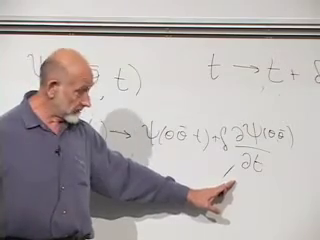
\includegraphics[width=0.72\textwidth]{lecture_05_figure_04.png}
\lectureframe{01:13:15.060}
\caption{Le tableau place \(t\to t+\delta\) au-dessus de la variation au premier ordre de \(\Psi\), en indiquant directement le terme dérivé.}
\end{figure}

\subsection{Translation dans une direction impaire}

Imaginons maintenant une transformation qui décale une coordonnée impaire :
\begin{equation}
\theta\longmapsto\theta+\epsilon,
\end{equation}
où \(\epsilon\) est un autre paramètre de Grassmann impair. Simultanément, faisons subir au temps un déplacement pair nilpotent,
\begin{equation}
t\longmapsto t+i\bar\theta\epsilon.
\end{equation}
\(\bar\theta\) et \(\epsilon\) sont tous deux impairs, si bien que leur produit est pair et peut être ajouté de façon cohérente à la coordonnée paire \(t\).

En plaçant le paramètre à gauche,
\begin{equation}
i\bar\theta\epsilon=-i\epsilon\bar\theta.
\end{equation}
la variation induite est donc
\begin{align}
\delta_\epsilon\Psi
&=\epsilon\,\partial_\theta\Psi
-i\epsilon\bar\theta\,\partial_t\Psi\\
&=\epsilon q_0\Psi,
\end{align}
où
\begin{equation}
q_0=\partial_\theta-i\bar\theta\partial_t.
\end{equation}
Cet opérateur différentiel impair engendre le déplacement combiné. Un générateur conjugué compatible, utilisant des dérivées à gauche, est
\begin{equation}
\bar q_0=-\partial_{\bar\theta}
+i\theta\partial_t.
\end{equation}

Les signes exacts dépendent du choix de dérivées de Grassmann à gauche ou à droite et de la façon dont la conjugaison inverse les facteurs impairs. En revanche, la fermeture sur les translations temporelles doit être indépendante de la convention. Avec les définitions ci-dessus,
\begin{align}
\{q_0,\bar q_0\}
&=i\{\partial_\theta,\theta\}\partial_t
+i\{\bar\theta,\partial_{\bar\theta}\}\partial_t\\
&=2i\partial_t.
\end{align}
Le terme dérivée-dérivée s’annule, de même que le terme quadratique en les coordonnées impaires. Les deux termes mixtes contribuent chacun \(i\partial_t\).

Puisque \(H=i\partial_t\) sur les états dans la représentation de Schrödinger,
\begin{equation}
\{q_0,\bar q_0\}=2H.
\end{equation}
Si nous normalisons les générateurs comme suit :
\begin{equation}
q=\frac{q_0}{\sqrt2},
\qquad
\bar q=\frac{\bar q_0}{\sqrt2},
\end{equation}
alors
\begin{equation}
\boxed{\{q,\bar q\}=H.}
\end{equation}
\editorialnote{Le cours traite délibérément les signes incertains, puis remarque l’apparition d’un facteur deux. La convention affichée, avec des dérivées à gauche, préserve ce calcul fait en classe tout en fixant une normalisation cohérente. D’autres conventions usuelles déplacent les signes entre les décalages des coordonnées et les générateurs.}

\begin{classroomqa}
\audiencequestion{D’où vient le facteur deux final dans l’anticommutateur du superspace ? \lecturetimestamp{01:24:21}}
\lecturerresponse{Il y a deux contributions mixtes égales. L’une vient de \(\{\partial_\theta,\theta\}=1\), l’autre de \(\{\partial_{\bar\theta},\bar\theta\}=1\). Chacune multiplie la dérivée temporelle. Les générateurs non normalisés donnent donc \(2i\partial_t\) ; un facteur \(1/\sqrt2\) dans chaque charge supersymétrique rétablit la normalisation précédente.}
\end{classroomqa}

\begin{classroomqa}
\audiencequestion{La construction repose-t-elle sur l’hypothèse que \(\epsilon\) est petit ? \lecturetimestamp{01:24:51}}
\lecturerresponse{Elle repose sur la nilpotence, non sur une grandeur numérique ordinaire. Puisque \(\epsilon^2=0\), tout développement en un seul \(\epsilon\) s’arrête après le premier ordre. Le qualifier d’infinitésimal ou de petit est une analogie utile, mais la troncature est exacte.}
\end{classroomqa}

\editorialnote{Les paramètres de Grassmann n’ont pas de grandeur positive ordinaire. Leur rôle de paramètres infinitésimaux découle de la nilpotence et de l’arrêt exact du développement.}

\subsection{Signification géométrique}

L’algèbre possède maintenant deux réalisations équivalentes. Dans la représentation par oscillateurs, \(Q\) et \(\bar Q\) remplacent les fermions par des bosons et les bosons par des fermions. Dans la représentation géométrique, \(q\) et \(\bar q\) translatent une fonction selon des directions impaires tout en induisant un décalage temporel ordinaire. Dans les deux représentations,
\begin{equation}
\begin{gathered}
\{\text{supercharge},\text{conjugate supercharge}\}\\
=\text{time-translation generator}.
\end{gathered}
\end{equation}

L’espace des coordonnées généralisées qui contient \(t,\theta,\bar\theta\) est le superspace. Dans une théorie relativiste des champs, il contient aussi les coordonnées spatiales ordinaires, et les charges supersymétriques se ferment sur la quantité de mouvement complète de l’espace-temps \(P_\mu\), et pas uniquement sur \(H=P_0\). Courber cette structure conduit vers la supergravité.

D’un certain point de vue, les variables de Grassmann sont un outil efficace pour organiser les bosons et les fermions. D’un autre, la relation de fermeture exprime une idée bien plus profonde : la distinction entre le type de particule et la géométrie de l’espace-temps n’est plus absolue. Deux déplacements dans des directions impaires produisent un déplacement selon une direction ordinaire. La question de savoir si la nature réalise cette structure expérimentalement est distincte du fait mathématique que cette structure est cohérente, économique et remarquablement rigide.
